\documentclass{beamer}
\usetheme{default}

\usepackage[dutch]{babel}
\usepackage{graphicx}

\title{Activation Records (AR)}
\author{Tobias Lamote \& Tim Robensyn}

\begin{document}
	
\begin{frame}[plain]
    \maketitle
\end{frame}

\begin{frame}
	Wat zit er in een stack?
\end{frame}

\begin{frame}{Stack van het handboek}
	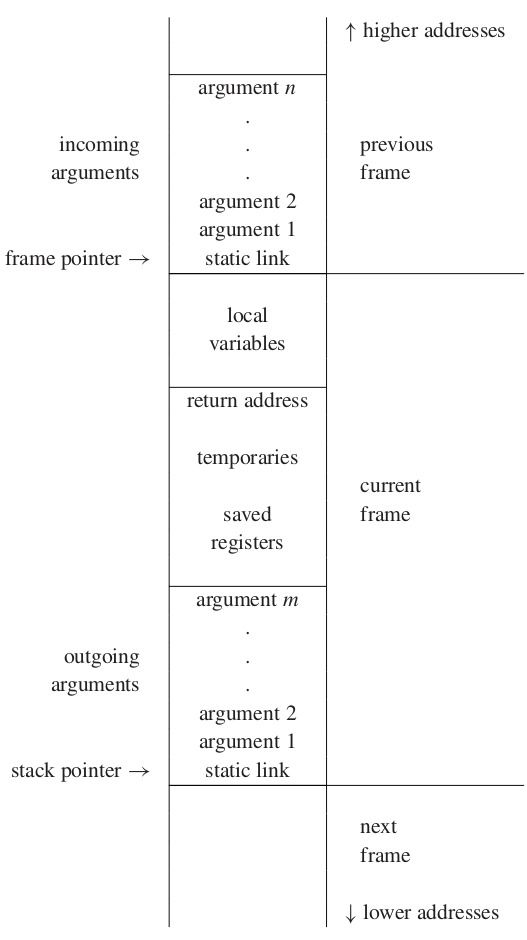
\includegraphics[height=\textheight]{theoretical_stack.png}
\end{frame}

% callee-save vs caller-save
% registers, escaping variables

\begin{frame}{Escaping variables}
	\begin{itemize}
		\item<1-> 
	\end{itemize}
\end{frame}

\begin{frame}{Demo: spelen met \texttt{gdb}}
	Examples:
	\begin{itemize}
		\item Functie die andere functie callt
		\item Functie met veel parameters (om spilling van de registers te demonstreren)
		\item Functie die stack overschrijft (hack hehe)
		\item Verschillende optimization levels testen (meer vars in registers? minder padding?)
	\end{itemize}
\end{frame}

\begin{frame}{Examenvragen}
	\begin{itemize}
		\item Gegeven een voorbeeldprogramma, kan dit programma activation records gebruiken die toegewezen zijn op een stack? Waarom?
		\item Leg uit hoe het doorgeven van parameters via de registers zorgt voor efficiënter geheugengebruik.
		\item Welk probleem lost call-by-reference op?
	\end{itemize}
\end{frame}

\section{Stacks voor gevorderden}
\begin{frame}{Spaghettistack}
	Wat met continuations?
	Voorbeeld
\end{frame}

\begin{frame}{Tail call optimization}
	Stack overflow is not just a website...
\end{frame}

\end{document}
